
% INSTRUCTIONS:
% To compile this file, run "latex HW_example";  you need to do it TWICE
%    to get the cross-references (to equations, etc) to show correctly.
% Figures can be included as shown below.  If you don't have a figure,
%    comment out those lines using % signs at the beginning of each line,
%    or else just keep hitting RETURN when LaTeX gives an error message
%    saying that it can't find the figure file.
% Run "dvips HW_example.dvi" to make a Postscript file HW_example.ps,
%    and then "ps2pdf HW_example.ps" to make a PDF file HW_example.pdf.

\documentclass[12pt]{article}
\usepackage{graphicx,indentfirst}
\usepackage{amsmath}

\pagestyle{plain}
\baselineskip 18pt
\textwidth 6.5in
\textheight 7.8in
\oddsidemargin 0.1in
\evensidemargin 0.1in
\topmargin 0.3in

\newcommand{\be}{\begin{equation}}
\newcommand{\ee}{\end{equation}}
\newcommand{\reff}[1]{(\ref{#1})}


\begin{document}

\title{Computational Physics \\ Homework 10}
\author{Yi-Hsuan Hsu}
\date{12/10/2014}
\maketitle

\section{Problem}
The structure of a material consist of a single dipole per lattice site is called the Ising Model. This simplified description of ferromagnet determined the overall magnetization of material by the number of dipoles that are aligned parallel to one-another. That is
\begin{equation}
	M = \Sigma \sigma_i
\end{equation}
Monte Carlo method with single -site Metropolis Algorithm is implemented to demonstrate Ising model with $L \times L$ lattice with periodic boundary condition.

\subsection{Algorithms}
The initial condition start with either "Hot" or "Cold". That is, a random arrangement of spin and all spin up. In each monte carlo step, we randomly flip single sspin in the lattice site and calculate the energy change of the system. The Hamiltonian of single spin in the lattice is
\begin{equation}
	\varepsilon=-\Sigma \sigma_i\sigma_j
\end{equation}
if the energy becomes lower, we accept the step. Other, we accept step with certain probability depends on temperature of system. The probability is writing in following form
\begin{equation}
	\frac{P(f->f')}{P(f'->f)}=\frac{e^{\frac{E_2}{T}}}{e^{\frac{E_1}{T}}}=e^{\beta\delta E}
\end{equation}
$\beta=\frac{1}{T}$. We determining a random number x between zero and one, if the ratio is greater than x than accept. Otherwise, we reject it and keep original state. Repeat this "dice-rolling" process, we obtain a sequence of iteration to $1.2 \times 10^5$steps. 

The statistical property of this chain can be observe by autocorrelation function and autocorrelation time. The autocorrelation function describe how close the markove chain converge to stationary state, or equalibrium. Define unnormalized autocorrlation function 
\begin{equation}
	C_{ff}(t)=\langle f_s f_{s+t}\rangle- \langle f_t \rangle^2
\end{equation}
The normalized autocorrelation function is then
\begin{equation}
	\rho_{ff}(t)=C_{ff}(t)/C_{ff}(0)
\end{equation}
A stationary state would converge to a constant value. Otherwise, it would fluctuate or even never converge.

More, there are exponential autocorrlation time and integrated autocorrelation time. Exponential autocorrelation time, noted $\tau_{exp}$, required to fit exponential decay $(~e^{\frac{-|t|}{\tau}})$ of $\rho(t)$ to $t\rightarrow\inf$, which is basically impossible to acquire. Instead, in a finite markov chain one can calculate $\tau_{int}$ by 
\begin{equation}
	\tau_{int}=\frac{1}{2} \sum_{t=-(n-1)}^{n-1} \lambda(t) \rho(t)
\end{equation}
$\lambda(t)$ represent for a windows region that remains signal we want. Others, we discards them as 
noise.

\[
\lambda(t)= 
\begin{cases}
1,& \text{if } |t|\leq M\\
0,              |t|& \geq M
\end{cases}
\]

where $M$ is a suitablely chosen cutoff, typically $M\geq 5\tau_{int}(M)$.


\subsection{Code description}
\subsubsection{Efficiency}
An initial version of my code using $for...loop$ in python to generate markov chain  and calculate the autocorrelation function. When running $10^{5}$ steps with $L=64$, it takes me almost an hour to generate markov chain and another hour to calculating autocorrelation function. And there are 300 sample need to do. It is totally impossible to do the job. 
\begin{eqnarray}
&&for\ t\ in\ range(nstep):\nonumber\\
	&&for\ k\ in\ range(0, nstep-t)\nonumber\\
		&&correlation+= Energy(t)*Energy(t+k)\nonumber\\
	&&autocorrelation(t)=sum(correlation)/(nstep-t)
\end{eqnarray}
Then I remembered there is once in recitation Geoff mentioned python broadcasting notation. I try to rewrite the summation of energy and autocorrelation function part. It runs 300 times faster than i do before. It just amazing speed that python achieved!
\begin{eqnarray}
autocorrelation(t)=sum(Energy[:nstep-t]*Energy[t:nstep])/(nstep-t)
\end{eqnarray}
Its really powerful.


\subsection{Sample output}

\subsubsection{$\varepsilon(t),M(t),M(t)^2$}
\begin{figure}[h!]
	\begin{center}
		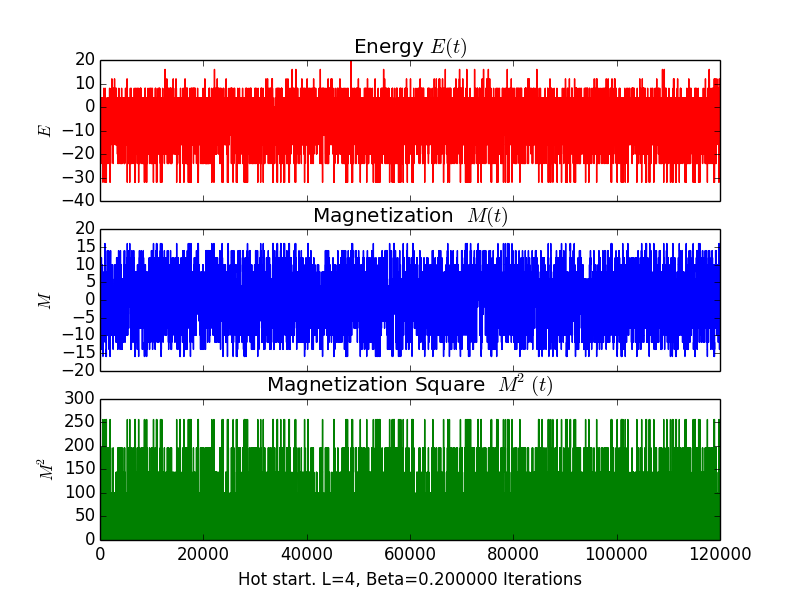
\includegraphics[width=0.4\textwidth]{exp1/Hot_L_4_Beta_2_iter_120000.png}
		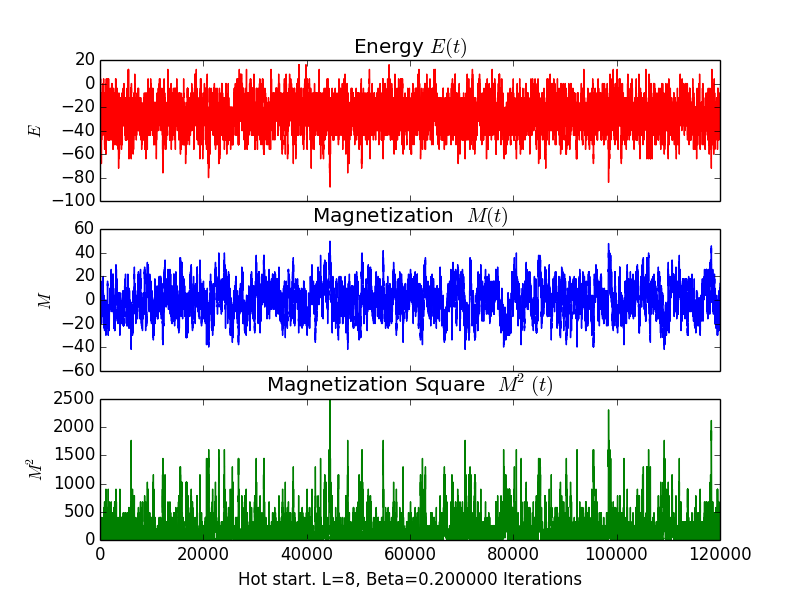
\includegraphics[width=0.4\textwidth]{exp1/Hot_L_8_Beta_2_iter_120000.png}
		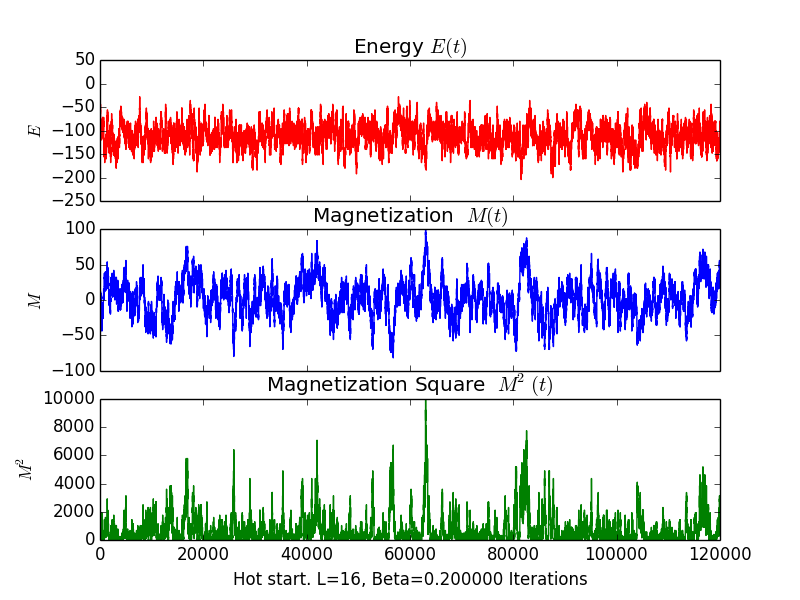
\includegraphics[width=0.4\textwidth]{exp1/Hot_L_16_Beta_2_iter_120000.png}
		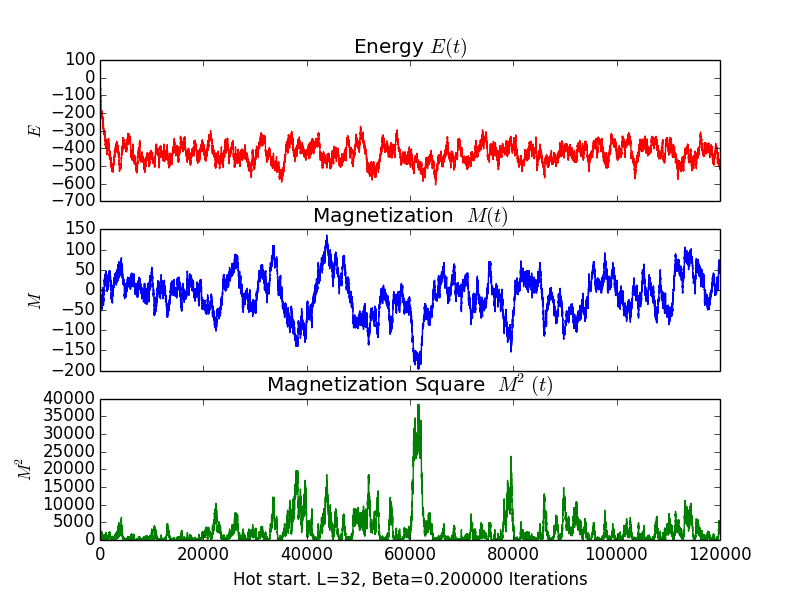
\includegraphics[width=0.4\textwidth]{exp1/Hot_L_32_Beta_2_iter_120000.png}
		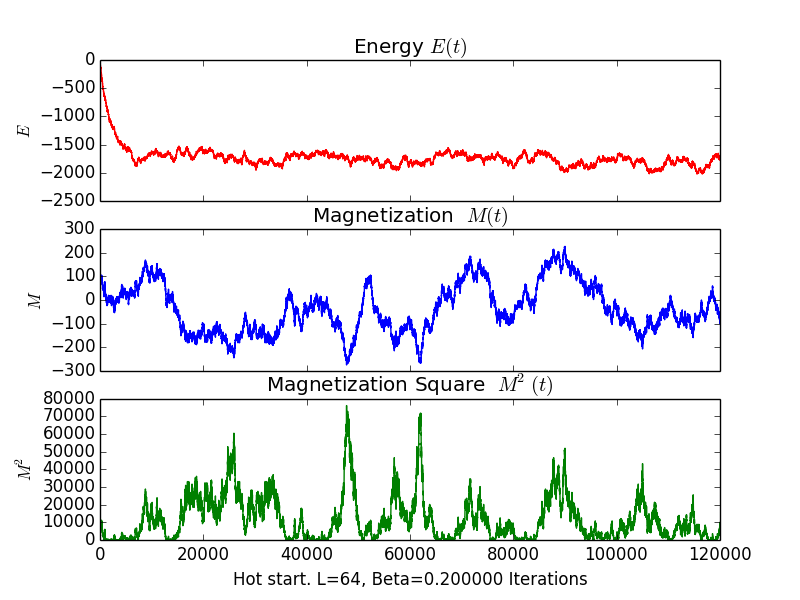
\includegraphics[width=0.4\textwidth]{exp1/Hot_L_64_Beta_2_iter_120000.png}
		\caption{Example of iteration for $\beta = 0.2$, Hot start, L=4,8,16,32,64.}
		\label{fig1}
	\end{center}
\end{figure}
Fig.1 shows the iteration series for $\beta=0.2$ with random initial condition. When L is small, there are only few available value of thos observable. Therefore, the series is crowded. When L is larger, we can see clearly the fluctuation of series. The Total energy goes to lower level whil magnetization fluctuate largely, which consist with our expectation due to the high temperature.

\begin{figure}[h!]
	\begin{center}
		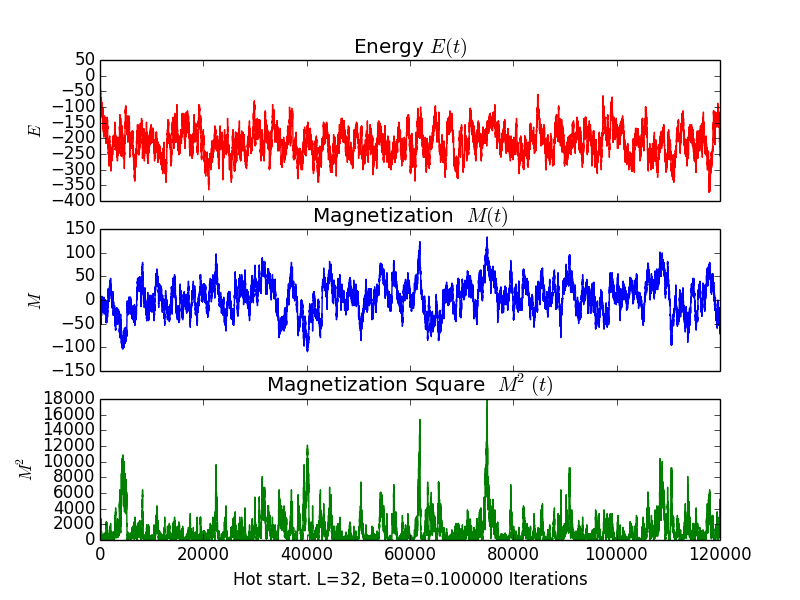
\includegraphics[width=0.4\textwidth]{exp1/Hot_L_32_Beta_1_iter_120000.png}
		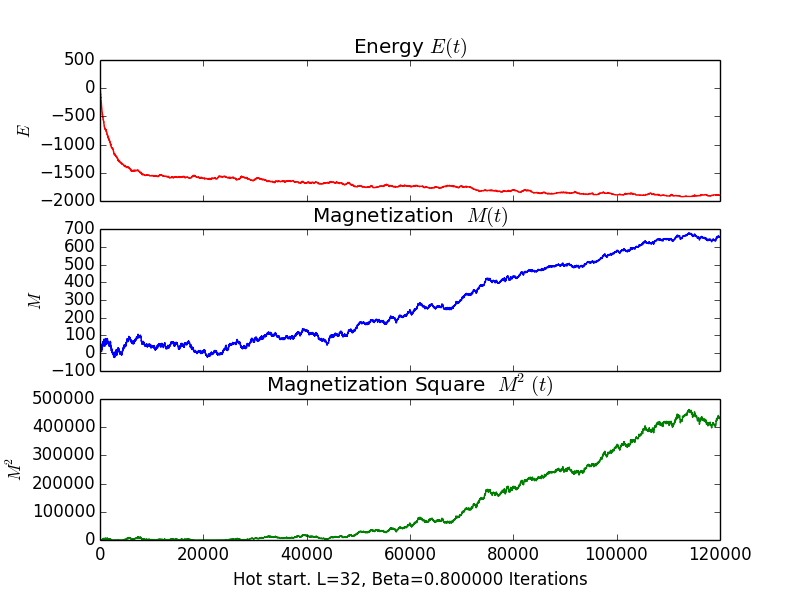
\includegraphics[width=0.4\textwidth]{exp1/Hot_L_32_Beta_8_iter_120000.png}
		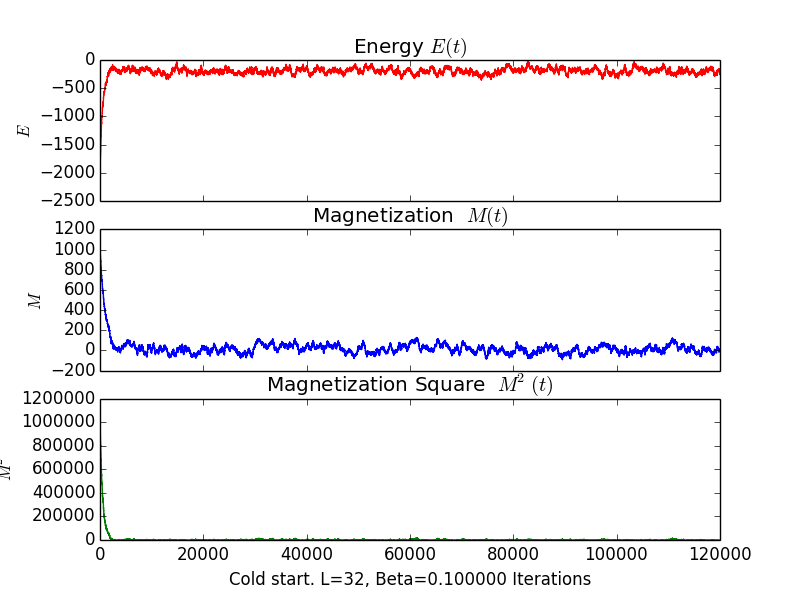
\includegraphics[width=0.4\textwidth]{exp1/Cold_L_32_Beta_1_iter_120000.png}
		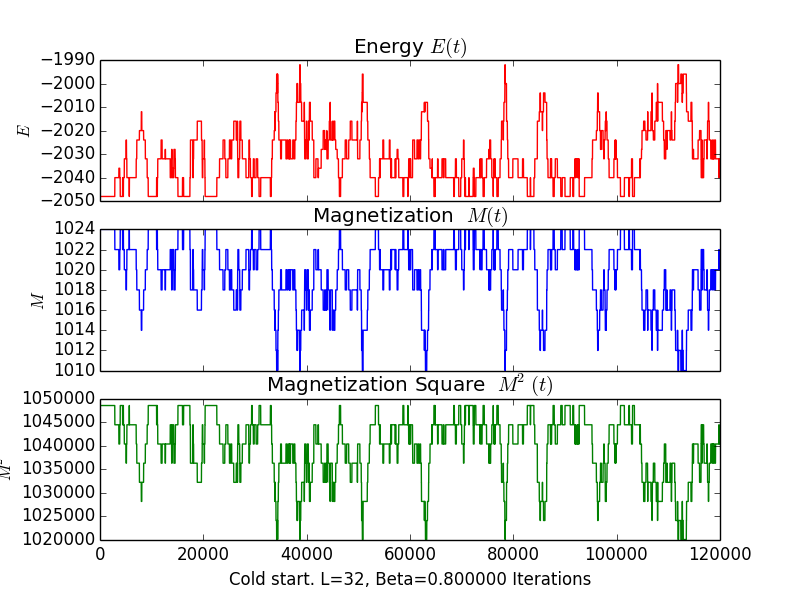
\includegraphics[width=0.4\textwidth]{exp1/Cold_L_32_Beta_8_iter_120000.png}
		\caption{}
		\label{fig2}
	\end{center}
\end{figure}
Fig.2 illustrates the series with hot and cold initial condition behave in small and large $\beta$. At small $\beta$ the observable fluctuate largely. In the other hand, observables transit to a stationary state quickly. A interesting result here is that the final state goes to zero magnetization state. It seems environment heat the system and break the parallel aligned spin structure.

At large value of $\beta$, the Hot start cooling down and stable in a low energy and highly magnetized state. The cold start stays almost the same as initial state when the series go far.

\subsubsection{$<E>,<M>,<M^2>$ and Autocorrelation function}
Fig.3 demonstrates the average value of observable in different temperature. The result consist with our expectation. The lower the temperature is, the higher the magnetized state belong to. 

\begin{figure}[h!]
	\begin{center}
		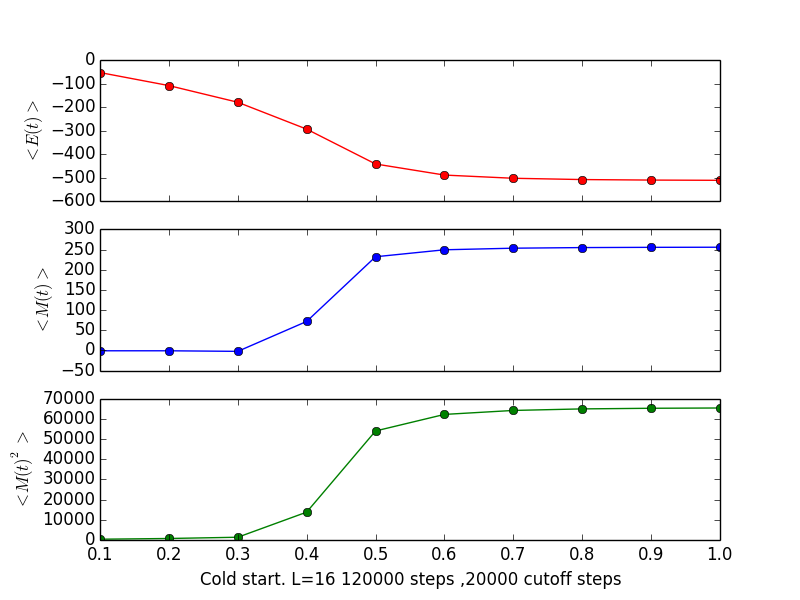
\includegraphics[width=0.4\textwidth]{average_plot_L_16_Cold.png}
		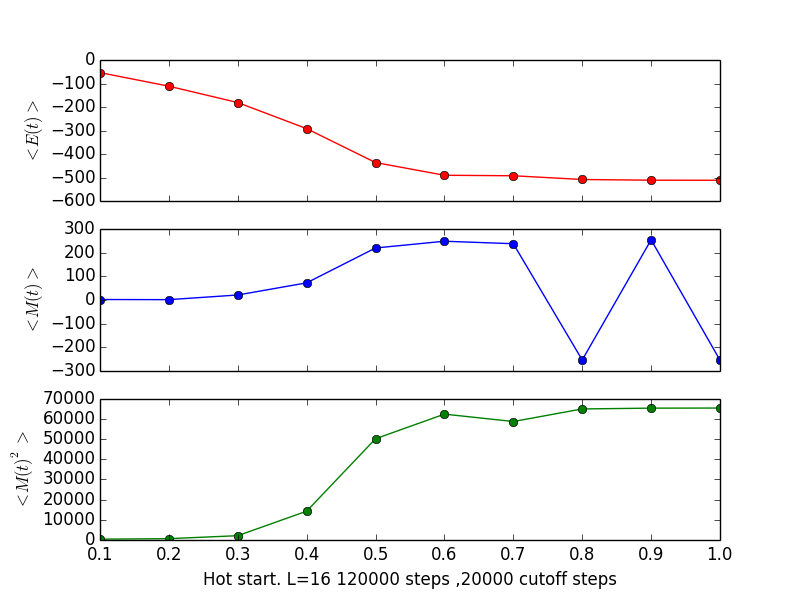
\includegraphics[width=0.4\textwidth]{average_plot_L_16_Hot.png}
		\caption{Average of observable in different temperature.}
		\label{fig3}
	\end{center}
\end{figure}

Fig.4 is the autocorrelation function with different lattice size. After a short exponential decay at the beginning, the correlation function enter to fluctuated state. When L become large, the fluctuation period is longer and amplitude is larger.

\begin{figure}[h!]
	\begin{center}
		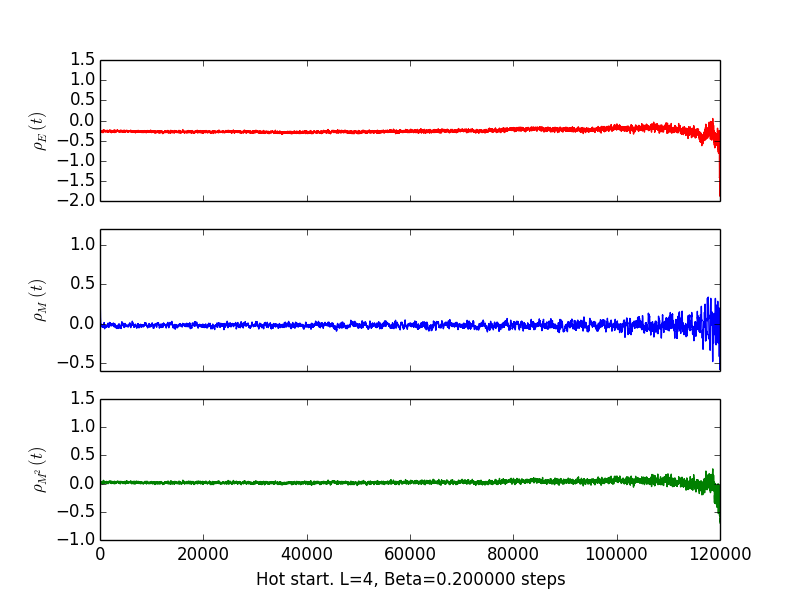
\includegraphics[width=0.4\textwidth]{exp2/Hot_L_4_Beta_2_iter_120000.png}
		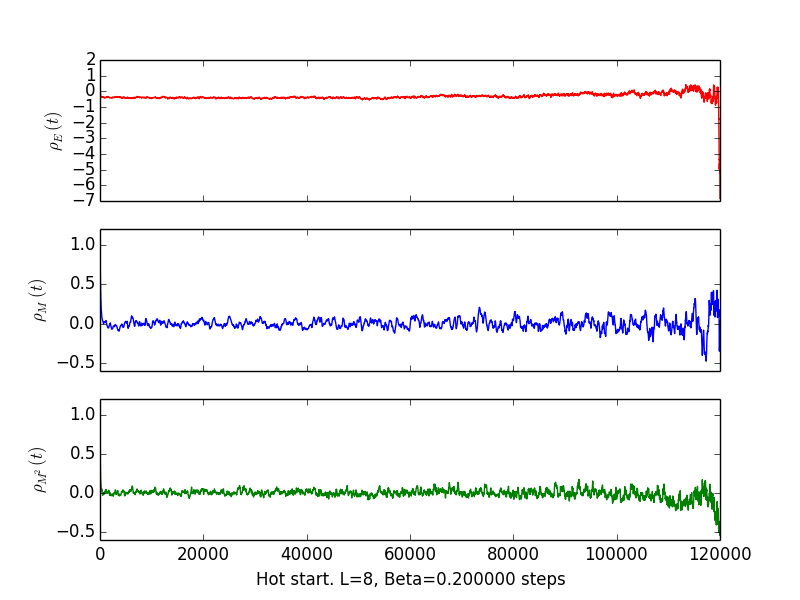
\includegraphics[width=0.4\textwidth]{exp2/Hot_L_8_Beta_2_iter_120000.png}
		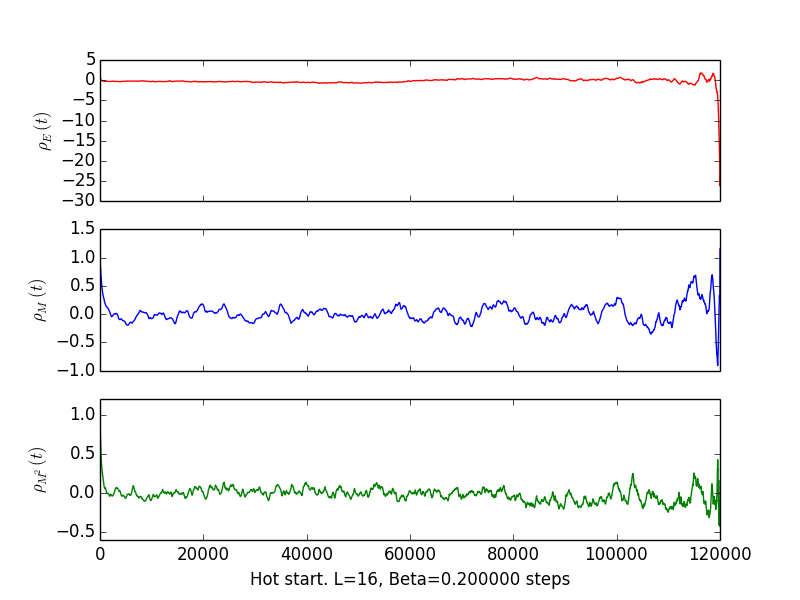
\includegraphics[width=0.4\textwidth]{exp2/Hot_L_16_Beta_2_iter_120000.png}
		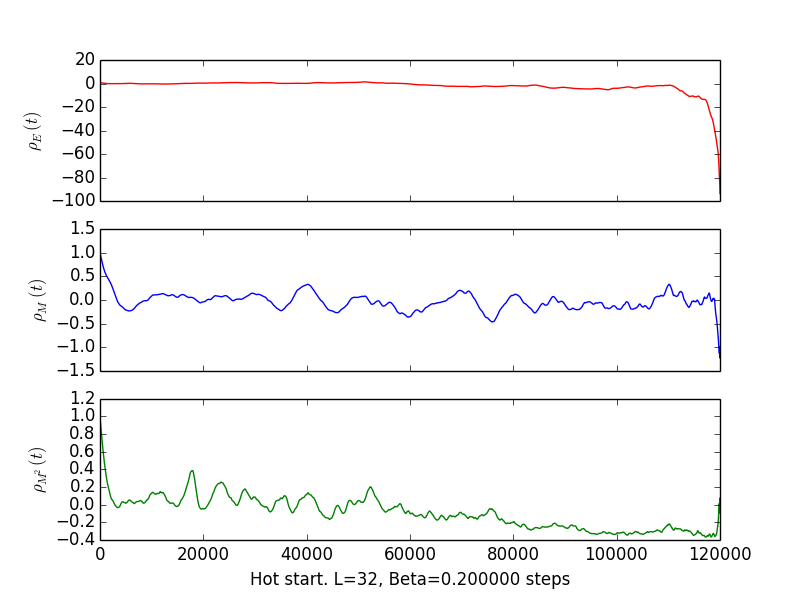
\includegraphics[width=0.4\textwidth]{exp2/Hot_L_32_Beta_2_iter_120000.png}
		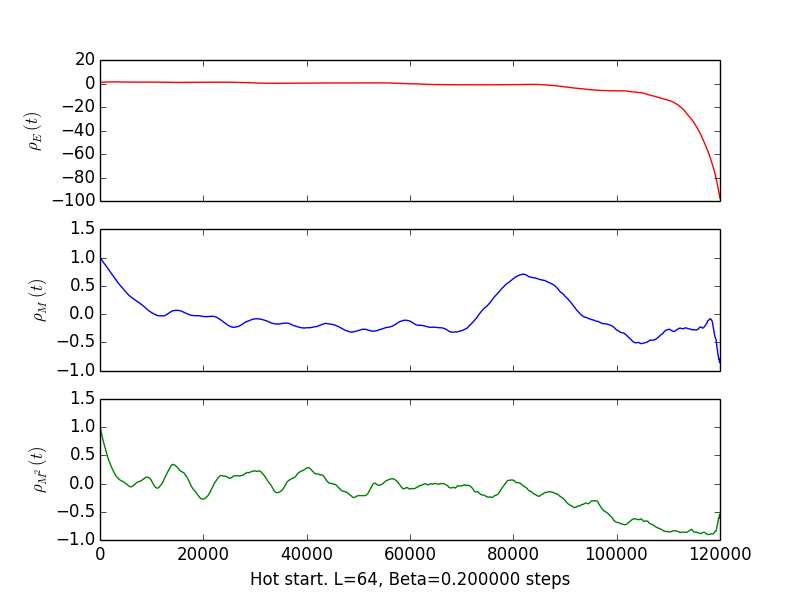
\includegraphics[width=0.4\textwidth]{exp2/Hot_L_64_Beta_2_iter_120000.png}
		\caption{Autocoerrelation function in different lattice size.}
		\label{fig4}
	\end{center}
\end{figure}

\subsubsection{$\tau_{int}(\beta,L)$}
$\tau_{int}$ provide an estimation of how fast the series converge to stationary state. Before critical $\beta$, we can clearly see the exponential growing up of $\tau$ in each $L$. Also, $\tau$ grows up linearly with lattice size $L$ with in the same temperature. We expect that the dependency of $\tau$ would break after the critical point. This phenomenon is illustrated in the figure both hot and cold initial condition. 

\begin{figure}[h!]
	\begin{center}
		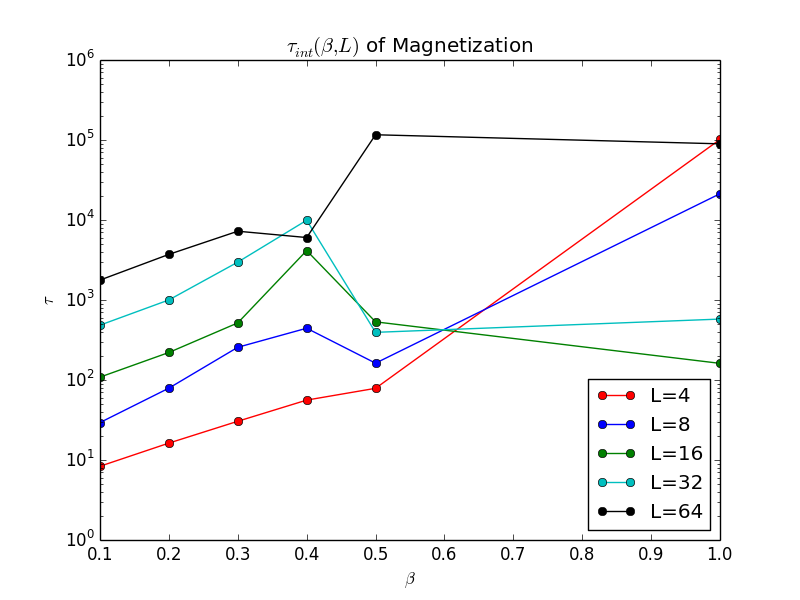
\includegraphics[width=0.4\textwidth]{Cold_Mag_sq.png}
		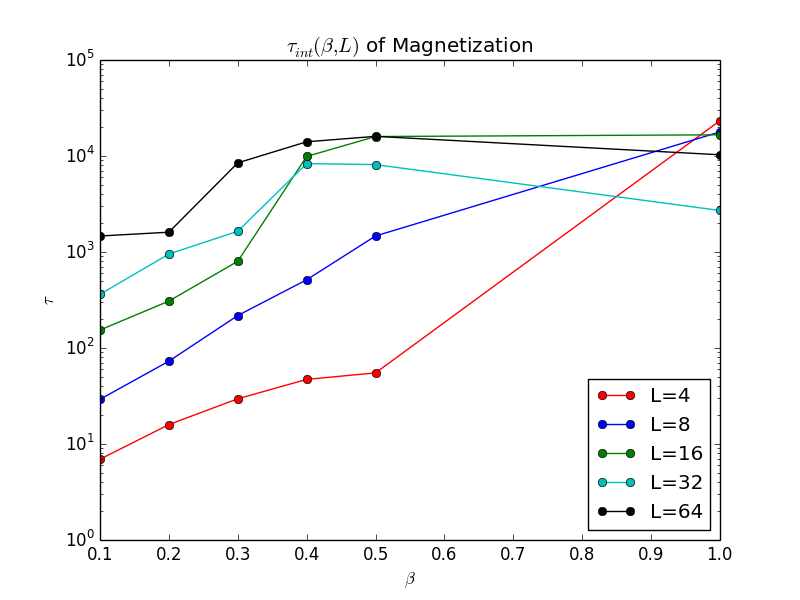
\includegraphics[width=0.4\textwidth]{Hot_Mag_sq.png}
		\caption{$\tau_{int}$ as a function of $\beta$ and $L$. LHS: Cold initial condition. RHS: Hot initial condition.}
		\label{fig5}
	\end{center}
\end{figure}



\subsubsection{Magnetic susceptibility $\chi$}
Fig.6 demonstrates the susceptability as a function of $L$. Magnetic susceptibility os a constant that indicate the degree of magnetization od a material in response to an applied magnetic field. At critical point, susceptibility should increase to infinite and decrease rapidly near critical point. 
Therefore, the results show that $\chi$ is propotional to L in order of 2. Because the volume is $L^{-2}$ and $<M^2> ~ L^4$.

\begin{figure}[h!]
	\begin{center}
		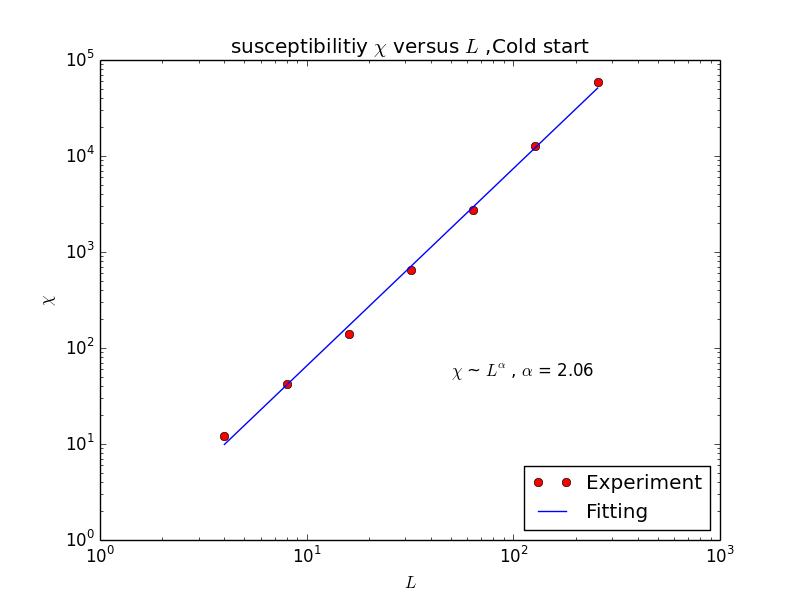
\includegraphics[width=0.4\textwidth]{Cold_susceptability.png}
		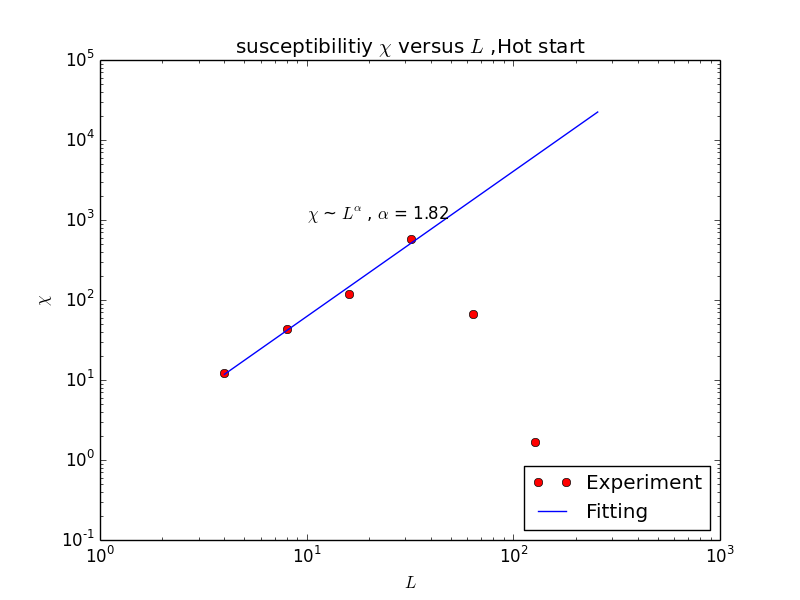
\includegraphics[width=0.4\textwidth]{Hot_susceptability.png}
		\caption{Susceptibility as a function of $L$. LHS: Cold start. RHS:Hot start}
		\label{fig6}
	\end{center}
\end{figure}

\end{document}



\begin{figure}[h!]
	\begin{center}
		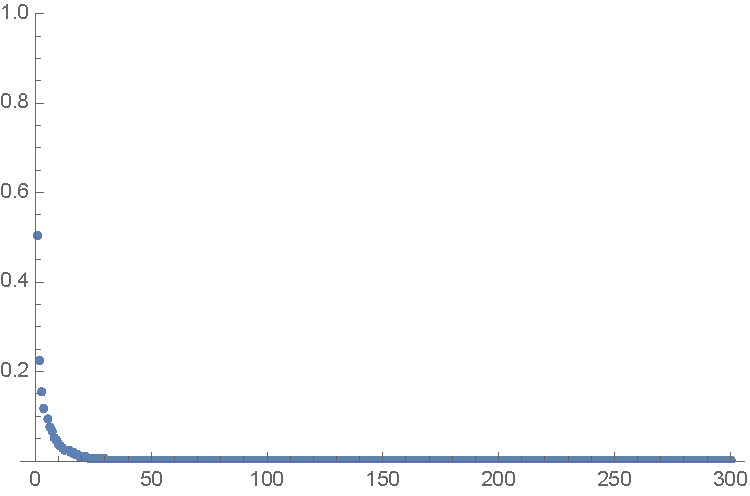
\includegraphics[width=0.4\textwidth]{a_09.pdf}
		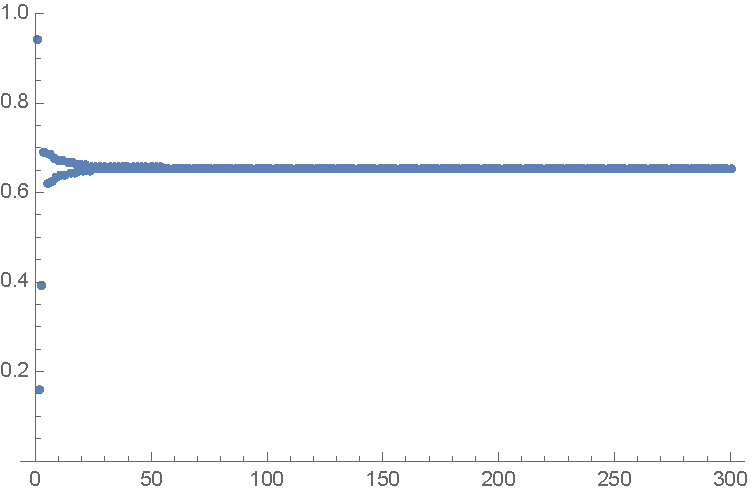
\includegraphics[width=0.4\textwidth]{a_29.pdf}
		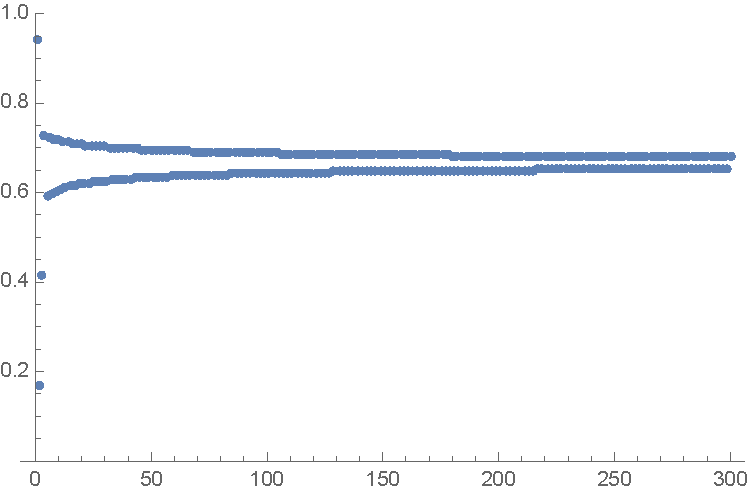
\includegraphics[width=0.4\textwidth]{a_30.pdf}
		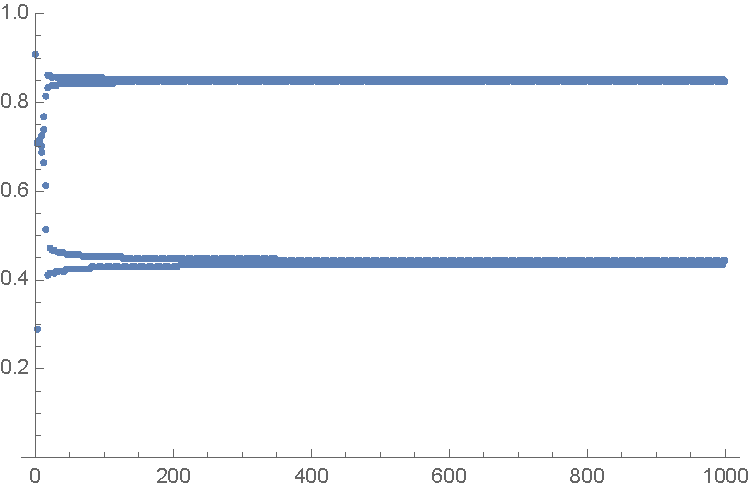
\includegraphics[width=0.4\textwidth]{a_3449.pdf}
		\caption{logistic map. Upper, left a=0.99, right a=2.9. Lower, left a=3.0, right a=3.4494.}
	\end{center}
\end{figure}

\begin{figure}[b!]
	\begin{center}
		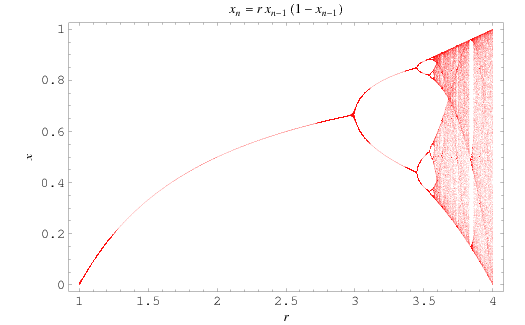
\includegraphics[width=0.8\textwidth]{logistic_map.png}
		\caption{bifurcation diagram of the logistic map. Pic. from Mahtworld}
		\label{fig1}
	\end{center}
\end{figure}


\begin{table}[h!]
	\begin{tabular}{c|lr}
		\hline
		A & $Table$ & Is\\ 
		Messy & To & Write\\
		\hline
	\end{tabular}
\end{table}


\begin{table}[h]
	\begin{center}
		\begin{tabular}{c|c}
			\hline
			period & bifurcation point a\\ 
			\hline
			2 & $0.7199616841972$ \\
			4 & $0.8332663532346$\\
			8 & $0.8591690091416$\\
			16& $0.8640801075000$*\\
			\hline
		\end{tabular}
	\end{center}
	\caption{Numerical approach to recursion sin function. First three are searching by bisection method, $\epsilon<10^{-10}$. *Last one is using step-in method, accuracy$\epsilon<10^{-5}$, although steps are much smaller than that.}
\end{table}

\begin{eqnarray}
G&&=6.67\times 10^{11} m^3 kg^{-1} s^{-2}\nonumber\\
M_{sun}&&=1.988\times 10^{30} kg\nonumber\\
c&&=3.0\times 10^8 ms^{-1}\nonumber\\
R_{orbit}&&=46\times 10^9 m\nonumber\\
v&&=58.98\times 10^3 ms^{-1}\nonumber\\
T_{period}&&=87.968 days
\end{eqnarray}



\begin{table}[b!]
	\begin{center}
		\begin{tabular}{c|c|c|c|c|c|c}
			\hline
			V-circle$(m_1,m_2)$ & $(3,1)$& $(3,2)$& $(3,3)$ & $(2,3)$ & $(1,3)$&$(0,3)$ \\ 
			\hline
			Eclipse Time $(s)$ & $ 2.018$&$1.990$&$2.212$ &$1.603$&$1.151$&$0.701$ \\
			\hline
			Convergence Rate (slope) & $0.305$& $0.356$& $0.384$& $0.444$& $0.571$&$0.774$\\
			\hline
			\hline
			W-circle$(m_1,m_2)$ & $(3,1)$& $(3,2)$& $(3,3)$ & $(2,3)$ & $(1,3)$&$(0,3)$ \\ 
			\hline
			Eclipse Time $(s)$ & $ 2.624$&$2.967$&$3.282$ &$2.226$&$1.896$&$1.2696$ \\
			\hline
			Convergence Rate (slope) & $0.357$& $407$& $0.454$& $0.618$& $0.611$&$0.774$\\
			\hline
		\end{tabular}
	\end{center}
	\caption{Table of eclipse time and convergence rate in each method by difference pre- and post- smoothing iteration.}
\end{table}